
\documentclass[border=10pt, 12pt]{standalone}
\usepackage[svgnames]{xcolor}
\usepackage{amsmath}
\usepackage{pgfplots}
\pgfplotsset{compat=newest}
\usepackage[sfdefault]{FiraSans}
\usepackage{FiraMono}
\renewcommand*\familydefault{\sfdefault}
\begin{document}
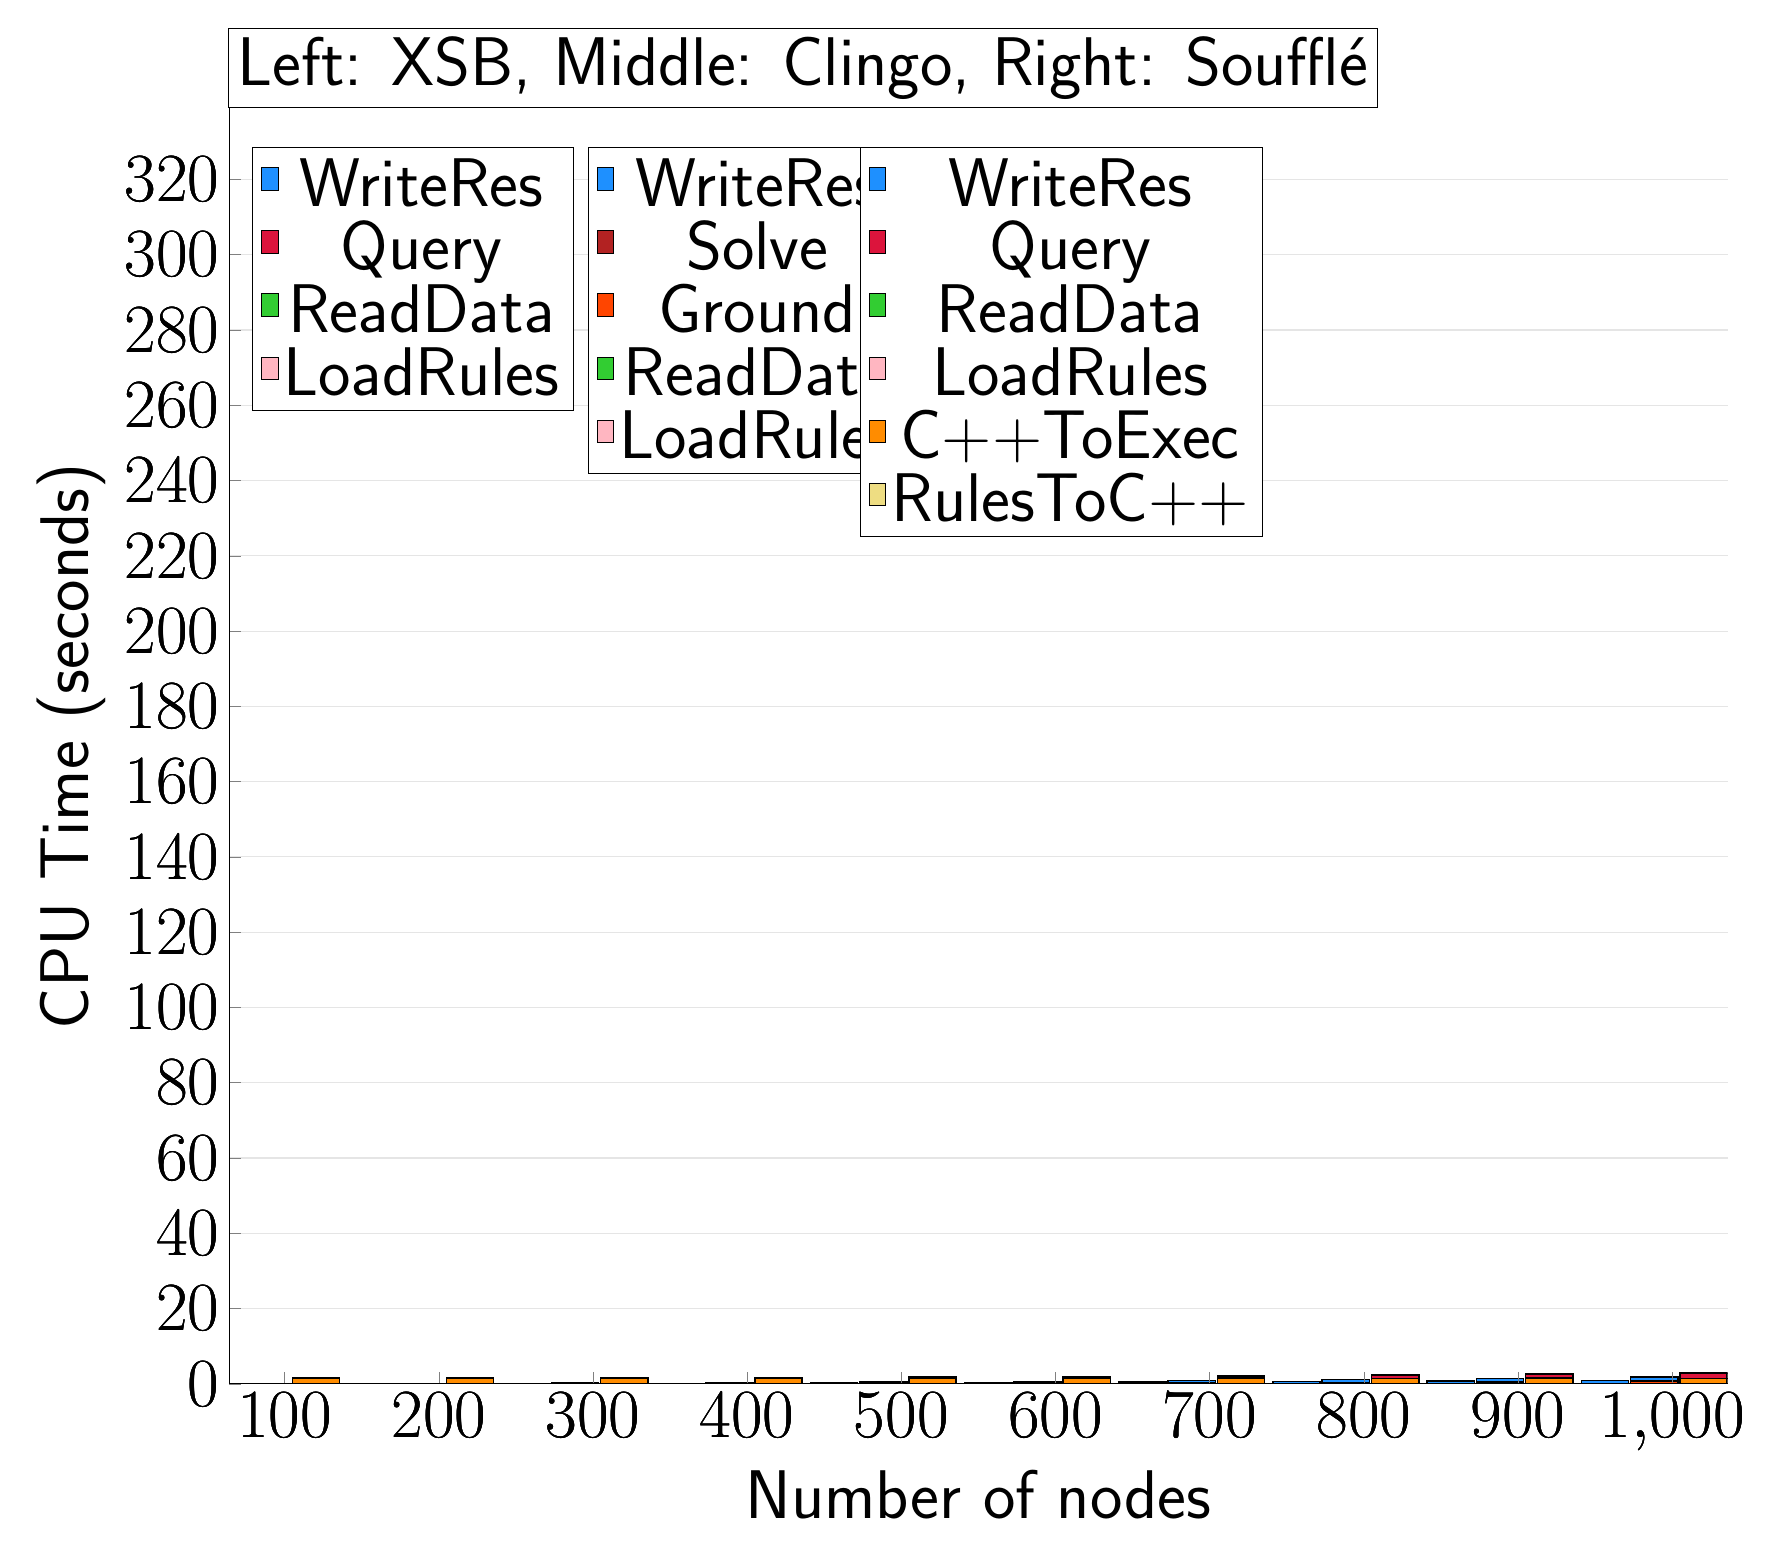
\begin{tikzpicture}
                        \begin{axis}[bar shift=-24.3pt, 
   ybar stacked,
   width=1.7\textwidth,
   bar width=0.6cm,
   ymajorgrids, tick align=inside,
   major grid style={draw=gray!20},
   xtick=data,
   ymin=0, ymax=338.8692,
   axis x line*=bottom,
   axis y line*=left,
   enlarge x limits=0.04,
   legend style={
       at={(0.23, 0.97)},
       anchor=north east,
       legend columns=1,
       font=\Huge,
   },
   ylabel={CPU Time (seconds)},
   xlabel={Number of nodes},
   label style={font=\Huge},
   tick label style={font=\Huge},
]
\addlegendimage{fill=DodgerBlue, draw=black, line width=0.2pt}
\addlegendentry{WriteRes}
\addlegendimage{fill=Crimson, draw=black, line width=0.2pt}
\addlegendentry{Query}
\addlegendimage{fill=LimeGreen, draw=black, line width=0.2pt}
\addlegendentry{ReadData}
\addlegendimage{fill=LightPink, draw=black, line width=0.2pt}
\addlegendentry{LoadRules}
\addplot +[fill=LightPink, draw=black, line width=0.55pt] coordinates {
(100, 0.0005486000000000004)
(200, 0.0005522000000000004)
(300, 0.0005488000000000009)
(400, 0.0005483999999999999)
(500, 0.0005510000000000002)
(600, 0.0005504000000000003)
(700, 0.0005486000000000002)
(800, 0.0005474)
(900, 0.0005610000000000001)
(1000, 0.0005510000000000002)
};
\addplot +[fill=LimeGreen, draw=black, line width=0.55pt] coordinates {
(100, 0.0001969999999999996)
(200, 0.00027820000000000004)
(300, 0.0003531999999999996)
(400, 0.00043619999999999976)
(500, 0.0005115999999999994)
(600, 0.0005971999999999994)
(700, 0.0006665999999999992)
(800, 0.0007473999999999998)
(900, 0.0008137999999999999)
(1000, 0.0008970000000000002)
};
\addplot +[fill=Crimson, draw=black, line width=0.55pt] coordinates {
(100, 0.0008534)
(200, 0.0033285999999999997)
(300, 0.007664800000000001)
(400, 0.0133718)
(500, 0.020749800000000002)
(600, 0.0306696)
(700, 0.041388)
(800, 0.053642600000000006)
(900, 0.06783380000000001)
(1000, 0.0833326)
};
\addplot +[fill=DodgerBlue, draw=black, line width=0.55pt] coordinates {
(100, 0.0084242)
(200, 0.03396199999999999)
(300, 0.075969)
(400, 0.134709)
(500, 0.20925699999999997)
(600, 0.29924019999999996)
(700, 0.4105905999999999)
(800, 0.5405052)
(900, 0.6745488)
(1000, 0.8266436)
};
\end{axis}

\begin{axis}[bar shift=-6.5pt, 
   ybar stacked,
   width=1.7\textwidth,
   bar width=0.6cm,
   ymajorgrids, tick align=inside,
   major grid style={draw=none},
   xtick=data,
   ymin=0, ymax=338.8692,
   axis x line*=none,
   axis y line*=none,
   enlarge x limits=0.04,
   legend style={
       at={(0.454, 0.97)},
       anchor=north east,
       legend columns=1,
       font=\Huge,
   },
   label style={font=\Huge},
   tick label style={font=\Huge},
]
\addlegendimage{fill=DodgerBlue, draw=black, line width=0.2pt}
\addlegendentry{WriteRes}
\addlegendimage{fill=FireBrick, draw=black, line width=0.2pt}
\addlegendentry{Solve}
\addlegendimage{fill=OrangeRed, draw=black, line width=0.2pt}
\addlegendentry{Ground}
\addlegendimage{fill=LimeGreen, draw=black, line width=0.2pt}
\addlegendentry{ReadData}
\addlegendimage{fill=LightPink, draw=black, line width=0.2pt}
\addlegendentry{LoadRules}
\addplot +[fill=LightPink, draw=black, line width=0.55pt] coordinates {
(100, 0.0)
(200, 0.0)
(300, 0.0)
(400, 0.0)
(500, 0.0)
(600, 0.0)
(700, 0.0)
(800, 0.0)
(900, 0.0)
(1000, 0.0)
};
\addplot +[fill=LimeGreen, draw=black, line width=0.55pt] coordinates {
(100, 0.0)
(200, 0.0)
(300, 0.0)
(400, 0.0)
(500, 0.0)
(600, 0.0)
(700, 0.0)
(800, 0.0)
(900, 0.0)
(1000, 0.0)
};
\addplot +[fill=OrangeRed, draw=black, line width=0.55pt] coordinates {
(100, 0.0020000000000000018)
(200, 0.020000000000000018)
(300, 0.04999999999999999)
(400, 0.08200000000000002)
(500, 0.15000000000000002)
(600, 0.20800000000000002)
(700, 0.29200000000000004)
(800, 0.374)
(900, 0.48200000000000004)
(1000, 0.624)
};
\addplot +[fill=FireBrick, draw=black, line width=0.55pt] coordinates {
(100, 0.0)
(200, 0.0)
(300, 0.0)
(400, 0.012000000000000007)
(500, 0.010000000000000009)
(600, 0.020000000000000018)
(700, 0.030000000000000034)
(800, 0.03800000000000004)
(900, 0.05800000000000005)
(1000, 0.06000000000000005)
};
\addplot +[fill=DodgerBlue, draw=black, line width=0.55pt] coordinates {
(100, 0.018000000000000016)
(200, 0.04999999999999999)
(300, 0.11800000000000006)
(400, 0.19)
(500, 0.288)
(600, 0.414)
(700, 0.566)
(800, 0.7399999999999999)
(900, 0.9099999999999999)
(1000, 1.152)
};
\end{axis}

\begin{axis}[bar shift=11.3pt, 
   ybar stacked,
   width=1.7\textwidth,
   bar width=0.6cm,
   ymajorgrids, tick align=inside,
   major grid style={draw=none},
   xtick=data,
   ymin=0, ymax=338.8692,
   axis x line*=none,
   axis y line*=none,
   enlarge x limits=0.04,
   legend style={
       at={(0.69, 0.97)},
       anchor=north east,
       legend columns=1,
       font=\Huge,
   },
   label style={font=\Huge},
   tick label style={font=\Huge},
]
\addlegendimage{fill=DodgerBlue, draw=black, line width=0.2pt}
\addlegendentry{WriteRes}
\addlegendimage{fill=Crimson, draw=black, line width=0.2pt}
\addlegendentry{Query}
\addlegendimage{fill=LimeGreen, draw=black, line width=0.2pt}
\addlegendentry{ReadData}
\addlegendimage{fill=LightPink, draw=black, line width=0.2pt}
\addlegendentry{LoadRules}
\addlegendimage{fill=DarkOrange, draw=black, line width=0.2pt}
\addlegendentry{C++ToExec}
\addlegendimage{fill=LightGoldenrod, draw=black, line width=0.2pt}
\addlegendentry{RulesToC++}
\addplot +[fill=LightGoldenrod, draw=black, line width=0.55pt] coordinates {
(100, 0.0020000000000000005)
(200, 0.004000000000000001)
(300, 0.0020000000000000005)
(400, 0.0)
(500, 0.006000000000000001)
(600, 0.0020000000000000005)
(700, 0.004000000000000001)
(800, 0.008000000000000002)
(900, 0.008000000000000002)
(1000, 0.006000000000000001)
};
\addplot +[fill=DarkOrange, draw=black, line width=0.55pt] coordinates {
(100, 1.4739999999999998)
(200, 1.48)
(300, 1.474)
(400, 1.472)
(500, 1.4759999999999998)
(600, 1.4819999999999998)
(700, 1.472)
(800, 1.4600000000000002)
(900, 1.4759999999999998)
(1000, 1.4440000000000004)
};
\addplot +[fill=LightPink, draw=black, line width=0.55pt] coordinates {
(100, 0.0001476)
(200, 0.00015179999999999998)
(300, 0.0001496)
(400, 0.0001652)
(500, 0.000163)
(600, 0.0001618)
(700, 0.0001558)
(800, 8.12e-05)
(900, 0.00015600000000000002)
(1000, 0.00010939999999999999)
};
\addplot +[fill=LimeGreen, draw=black, line width=0.55pt] coordinates {
(100, 0.0008078)
(200, 0.0012536000000000001)
(300, 0.0017402000000000001)
(400, 0.0020767999999999997)
(500, 0.0024128000000000005)
(600, 0.0027903999999999997)
(700, 0.0031616000000000005)
(800, 0.002354)
(900, 0.0038681999999999996)
(1000, 0.0026264)
};
\addplot +[fill=Crimson, draw=black, line width=0.55pt] coordinates {
(100, 0.0209322)
(200, 0.0641708)
(300, 0.12072559999999999)
(400, 0.2014522)
(500, 0.307495)
(600, 0.4401084)
(700, 0.5984076)
(800, 0.7799656)
(900, 1.0014732000000002)
(1000, 1.2455399999999999)
};
\addplot +[fill=DodgerBlue, draw=black, line width=0.55pt] coordinates {
(100, 0.0038132)
(200, 0.009432400000000002)
(300, 0.019483)
(400, 0.034599599999999994)
(500, 0.053508)
(600, 0.07685220000000001)
(700, 0.1043782)
(800, 0.1374724)
(900, 0.17306039999999995)
(1000, 0.2142228)
};
\end{axis}


\node[anchor=south, draw, fill=white] at (rel axis cs:0.42,1) {\Huge Left: XSB, Middle: Clingo, Right: Soufflé};
\end{tikzpicture}
\end{document}
                    